\section{Tính cấp thiết của đề tài}
Với sự bùng nổ của Internet trong những năm gần đây, các diễn đàn, trang web, mạng xã hội, v.v. dần trở nên phổ biến và tiếp cận được nhiều hơn tới mọi người. Thông qua các kênh thông tin này, chúng ta có thể tiếp cận và chia sẻ thông tin một cách nhanh chóng hơn bao giờ hết. Các trang web và mạng xã hội này có một lượng lớn người sử dụng từ đa dạng các thành phần xã hội khác nhau. Đồng thời nội dung trên Internet cũng ngày càng trở nên phong phú và khó đoán hơn. Mọi người ngày nay coi mạng xã hội không chỉ là một kênh phương tiện giải trí mà còn là nơi giao lưu và chia sẻ thông tin với nhau. Không chỉ người lớn mới sử dụng Internet và mạng xã hội, trẻ em ngày nay cũng được tiếp cận với Internet từ sớm để phục vụ nhu cầu học tập và giải trí. Tuy nhiên ngoài những lợi ích có thể thấy được, Internet mang lại những nguy cơ không lường trước được cho những em nhỏ, và một trong số đó là những ngôn từ không phù hợp trên Internet, hay còn gọi là ngôn ngữ độc hại.

Chỉ mới gần đây thôi, vào năm 2020, Việt Nam đã lọt vào Top 5 những nước kém văn minh nhất thế giới trên Internet \cite{webpage28}. Điều này chứng tỏ môi trường mạng Việt Nam tiềm ẩn nhiều nguy cơ cho những em nhỏ tiếp cận tới những ngôn ngữ không phù hợp với thuần phong mĩ tục, góp phần làm xấu đi hình ảnh đất nước trong mắt bạn bè quốc tế.

Nhằm góp phần ngăn chặn sự tiêu cực mà ngôn ngữ độc hại đem lại, nhóm chúng tôi xin đề xuất bài toán ``Nhận diện văn bản tiêu cực sử dụng học máy'' áp dụng cho tiếng Việt làm đề tài khoá luận tốt nghiệp cho mình.

\section{Mục tiêu và nhiệm vụ nghiên cứu}
Mục tiêu: Xây dựng được mô hình phát hiện các từ ngữ độc hại. Từ đó, áp dụng cho chatbot và tiện ích trong trình duyệt để hỗ trợ người dùng trong việc phát hiện và ngăn chặn ngôn ngữ độc hại.

Nhiệm vụ:
\begin{itemize}
    \item Tìm hiểu các kiến trúc mạng neuron và các thuật toán dùng trong xử lý văn bản.
    \item Tìm hiểu về xử lí ngôn ngữ tự nhiên.
    \item Tìm hiểu các kỹ thuật nhúng từ (word embedding).
    \item Tìm hiểu các thư viện, module hỗ trợ học máy và học sâu như Tensorflow, Sklearn, v.v..
    \item Tìm hiểu những kiến trúc học sâu như LSTM, RNN, Transformer, v.v. và các mô hình tiền huấn luyện GPT, BERT, v.v..
    \item Ứng dụng các kiến thức đã tìm hiểu vào việc xây dựng mô hình phát hiện từ ngữ độc hại.
    \item Áp dụng mô hình đã xây dựng vào những ứng dụng thực tiễn.
\end{itemize}

\section{Cách tiếp cận và phương pháp nghiên cứu}
% Cách tiếp cận:
% \begin{itemize}
%     \item Sử dụng các lý thuyết học máy, học sâu và kỹ thuật nhúng từ.
%     \item Sử dụng các thư viện, module hỗ trợ học máy và học sâu như Tensorflow, Sklearn, \dots
% \end{itemize}

% Phương pháp nghiên cứu:
% \begin{itemize}
%     \item Xử lí dữ liệu đầu vào trước khi thực hiện huấn luyện.
%     \item Huấn luyện và đánh giá mô hình dựa trên dữ liệu đầu vào để đánh giá khả năng phát hiện từ ngữ xấu của mô hình.
% \end{itemize}

\begin{figure}[htb]
    \centering
    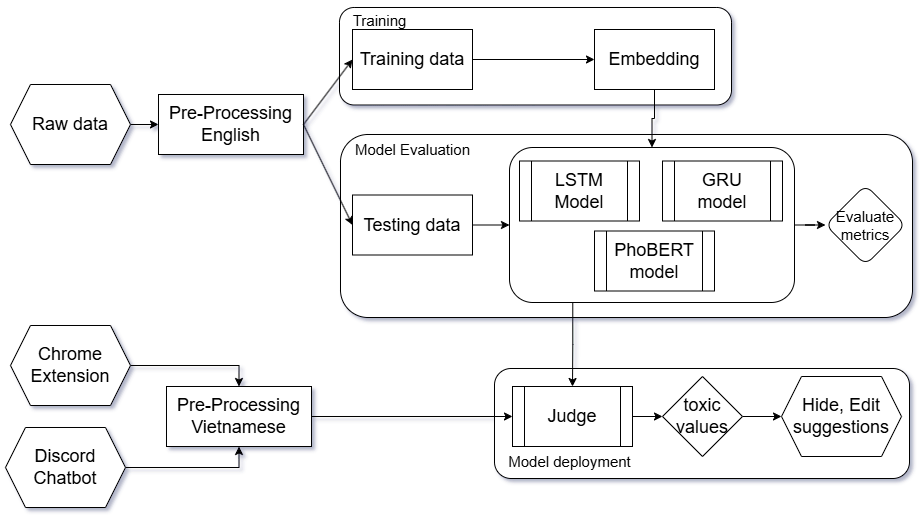
\includegraphics[width=\textwidth]{image/ToxicDetection_workflow.drawio.png}
    \caption{Phương pháp tiếp cận trong bài toán nhận diện ngôn ngữ độc hại}
    \label{figure:ToxicDetection_workflow}
\end{figure}

Kiến trúc tổng quan của hệ thống phát hiện văn bản độc hại được minh họa trong Hình \ref{figure:ToxicDetection_workflow}.

Hệ thống phân loại độc hại trong ngôn ngữ sẽ bắt đầu với một loạt các bước tiền xử lý dữ liệu để làm sạch và chuẩn hóa dữ liệu thành định dạng mà mô hình có thể hiểu được bao gồm hai kỹ thuật sẽ được sử dụng: phân tách từ (tokenization) và nhúng từ (word embedding).

Trong nhiệm vụ phân loại, chúng tôi xây dựng hai mô hình mạng thần kinh hồi quy sử dụng hai kiến trúc: LSTM và GRU như đã đề cập, và một mô hình được tinh chỉnh từ PhoBERT. Với hai mô hình mạng hồi quy, mỗi mô hình bao gồm sáu lớp: lớp đầu vào nhận dữ liệu đầu vào dưới dạng các token, lớp nhúng từ sử dụng fastText, lớp dropout ở giữa hai lớp mạng thần kinh hồi quy hai chiều để kiểm soát quá khớp (overfitting), và cuối cùng là lớp dense đánh giá mức độ độc hại của văn bản dựa trên các giá trị độc hại đã định nghĩa. Về mô hình PhoBERT, chúng tôi sử dụng mô hình đã được huấn luyện trước và thêm một lớp classifier vào phía sau tương ứng với sáu mức độ độc hại của văn bản.

Vì đối mặt với bài toán sử dụng ngôn ngữ tự nhiên, mô hình mạng thần kinh hồi quy hai chiều (bidirectional RNN) và PhoBERT được ưu tiên chọn lựa, trong khi mô hình fastText được coi là phù hợp nhất cho tiếng Việt.

Khi nhận dữ liệu thực tế từ các ứng dụng, hệ thống sẽ xử lý dữ liệu lần nữa trước khi đưa vào mô hình đánh giá. Tùy thuộc vào loại ứng dụng và yêu cầu về độ trễ của phản hồi, hệ thống sẽ sử dụng một trong ba mô hình để tối ưu hóa kết quả cuối cùng. Sau đó, cung cấp một số gợi ý chỉnh sửa nhằm đáp ứng các tiêu chuẩn của cộng đồng đối với Chatbot, hoặc ẩn văn bản tiêu cực trên trang web đối với Tiện ích Chrome.

\section{Phân tích những công trình có liên quan}

% [2] K. Dubey, R. Nair, M. U. Khan, and S. Shaikh, "Toxic comment detection using LSTM," in Proc. 2020 Third International Conference on Advances in Electronics, Computers and Communications (ICAECC), Dec. 2020, doi:10.1109/icaecc50550.2020.9339521.
% [3] A. K. Bala, “Toxic comments identification and classification using Deep Neural Networks,” Academia.edu, https://www.academia.edu/41458366/Toxic_Comments_Identification_and_Classification_Using_Deep_Neural_Networks (accessed Apr. 23, 2024).
% [4] R. Sharma and M. Patel, “Toxic comment classification using neural networks and machine learning,” IARJSET, vol. 5, no. 9, pp. 47–52, Sep. 2018. doi:10.17148/iarjset.2018.597
% [5] V. Maslej-Krešňáková, M. Sarnovský, P. Butka, and K. Machová, “Comparison of deep learning models and various text pre-processing techniques for the toxic comments classification,” Applied Sciences, vol. 10, no. 23, p. 8631, Dec. 2020. doi:10.3390/app10238631

Với tập dữ liệu gốc là văn bản Tiếng Anh, cách tiếp cận phổ biến trong bài toán này là sử dụng các mô hình học sâu chuyên biệt cho dữ liệu chuỗi và xử lý ngôn ngữ tự nhiên.

Như trong \cite{9339521}, các tác giả sử dụng các phương pháp phân tách từ (tokenization) kết hợp với mô hình học sâu LSTM. Cách tiếp cận này tạo ra một mô hình có kết quả khá cao, với độ chính xác (precision) đạt 94,49\%, độ nhạy (recall) đạt 92,79\% và độ chính xác (accuracy) đạt 94,94\%.

Một nghiên cứu khác sử dụng phiên bản tiên tiến hơn của Long Short-Term Memory (LSTM), là Bidirectional LSTM (BiLSTM), để cải thiện thêm độ chính xác của dự đoán \cite{webpage25}.

Ngoài việc chỉ sử dụng RNN, bài báo \cite{Sharma2018} còn sử dụng mạng nơ-ron tích chập (CNN) song song với mô hình LSTM. Mặc dù kết quả đánh giá cho thấy CNN cũng đạt được kết quả khá tốt, LSTM vẫn vượt trội hơn cả về độ chính xác lẫn hiệu suất thời gian khi sử dụng cùng số epoch.

Nghiên cứu \cite{app10238631} cho thấy rằng không chỉ việc áp dụng các mô hình phức tạp mà cả việc sử dụng các phương pháp tiền xử lý cơ bản và nhúng từ (word embedding) cũng có thể ảnh hưởng đến hiệu suất phân loại. Để chứng minh điều này, các tác giả đã tiến hành đánh giá thực nghiệm về kiến trúc kết hợp BiLSTM + CNN, mô hình ngôn ngữ BERT (Bidirectional Encoder Representation from Transformer) với các phương pháp tiền xử lý và nhúng từ khác nhau.

\section{Dự kiến kết quả đạt được}
Về lý thuyết: Nhóm mong muốn sau khi thực hiện nghiên cứu có thể học hỏi và hiểu sâu về nội dung lý thuyết của bài toán đã nêu. Đồng thời có cơ hội thực hành mô hình học sâu trong quá trình huấn luyện dữ liệu cho bài toán.

Về mặt sản phẩm: Nhóm mong muốn xây dựng được một mô hình có thể phát hiện các ngôn ngữ độc hại với một mức chính xác khả quan và có thể ứng dụng thực tế. Từ đó, áp dụng vào thực tiễn dưới dạng chatbot hoặc tiện ích trong trình duyệt để hỗ trợ người dùng trong việc phát hiện và ngăn chặn ngôn ngữ độc hại
